\documentclass{beamer}

\usepackage[utf8]{inputenc}
\usepackage{default}
\usepackage{amsmath}
\usepackage{tikz}
%\usepackage{chronology}
\usepackage{chronosys}
\usepackage{graphicx}
\usepackage{mwe} % for raisebox
\usepackage{subfig}
\usepackage{multirow}
\usepackage{makecell}%To keep spacing of text in tables
%\renewcommand\cellalign{cc}
\newcommand{\mlcell}[1]{\begin{tabular}{@{}c@{}}#1\end{tabular}}
\usepackage{tabularx} %To do vertical spacing
\usepackage{cellspace}
\setlength\cellspacetoplimit{1pt}
\setlength\cellspacebottomlimit{1pt}
\addparagraphcolumntypes{x, }
\graphicspath{ {./figures/} }

%%%%FROM
%%%%  https://tex.stackexchange.com/questions/312704/chronosys-not-using-only-years
\usepackage{datenumber,xparse}
\usetikzlibrary{arrows.meta,backgrounds}
\newcounter{chronosstartdate}
\newcounter{chronosenddate}
\newcounter{chronosstartyear}
\newcounter{chronosendyear}
\newcounter{chronosyeardate}
\newcounter{chronosthingdate}
\newcounter{chronosotherthingdate}
\pgfkeys{/pgf/number format,
  int detect,
  set thousands separator={},
}
\tikzset{
  chronos/.code={% https://tex.stackexchange.com/a/159856/ - Claudio Fiandrino
    \tikzset{%
      align=center,
      anchor=mid,
      /chronos/.cd,
      #1
    }%
    \setstartyear{\chronosstartyear}%
    \setmydatenumber{chronosstartdate}{\chronosstartyear}{\chronosstartmonth}{\chronosstartday}%
    \setmydatenumber{chronosenddate}{\chronosendyear}{\chronosendmonth}{\chronosendday}%
    \pgfmathsetmacro\chronosunit{(\chronoswidth-20pt)/(\thechronosenddate-\thechronosstartdate)}%
    \draw [line width=\chronosheight] (-10pt,0) coordinate (chronos pre) -- +(\chronoswidth,0) coordinate (chronos post);
    \coordinate (chronos start) at (0,0);
    \coordinate (chronos end) at ([xshift=-10pt]chronos post);
    \setcounter{chronosstartyear}{\chronosstartyear}%
    \setcounter{chronosendyear}{\chronosendyear}%
    \def\tempa{01}%
    \ifx\chronosstartmonth\tempa
      \ifx\chronosstartday\tempa
        \else\stepcounter{chronosstartyear}%
      \fi
      \else\stepcounter{chronosstartyear}%
    \fi
    \def\tempa{12}%
    \def\tempb{31}%
    \ifx\chronosendmonth\tempa
      \ifx\chronosendday\tempb
        \stepcounter{chronosendyear}%
      \fi
    \fi
    \foreach \i in {\thechronosstartyear,...,\thechronosendyear} {%
      \setmydatenumber{chronosyeardate}{\i}{01}{01}%
      \node [above, anchor=south, yshift=.5*\chronosheight] at ({(\thechronosyeardate-\thechronosstartdate)*\chronosunit pt},0) {\i}; }
  },
  chronos set date/.code args={#1-#2-#3:#4}{%
    \tikzset{%
      /chronos/.cd,
      #4 year={#1},
      #4 month={#2},
      #4 day={#3},
    }%
    \setmydatenumber{chronos#4date}{\csname chronos#4year\endcsname}{\csname chronos#4month\endcsname}{\csname chronos#4day\endcsname}%
  },
  chronos date/.style args={#1-#2-#3}{%
    chronos set date/.expanded={#1-#2-#3:thing}%
  },
  chronos period date/.style args={#1-#2-#3}{%
    chronos set date/.expanded={#1-#2-#3:otherthing}%
  },
  /chronos/.search also={/tikz},
  /chronos/.cd,
  start year/.store in=\chronosstartyear,
  start month/.store in=\chronosstartmonth,
  start day/.store in=\chronosstartday,
  end year/.store in=\chronosendyear,
  end month/.store in=\chronosendmonth,
  end day/.store in=\chronosendday,
  thing year/.store in=\chronosthingyear,
  thing month/.store in=\chronosthingmonth,
  thing day/.store in=\chronosthingday,
  otherthing year/.store in=\chronosotherthingyear,
  otherthing month/.store in=\chronosotherthingmonth,
  otherthing day/.store in=\chronosotherthingday,
  start date/.style args={#1-#2-#3}{%
    start year={#1},
    start month={#2},
    start day={#3},
  },
  end date/.style args={#1-#2-#3}{%
    end year={#1},
    end month={#2},
    end day={#3},
  },
  width/.store in=\chronoswidth,
  height/.store in=\chronosheight,
  period/.style={draw=gray},
  period event line/.style={draw=gray, -{Triangle[width=1.5pt, reversed, length=.75pt, fill=gray]}},
  period event/.style={anchor=north, fill=gray!25, draw=gray, rounded corners, align=center, font=\footnotesize},
  event line/.style={draw=gray, -{Triangle[width=1.5pt, reversed, length=.75pt, fill=gray]}},
  event/.style={anchor=north, fill=gray!25, draw=gray, rounded corners, align=center, font=\footnotesize},
  start date=1001-10-01,
  end date=1003-06-14,
  width=100mm,
  height=1pt,
  chronos date=1850-01-01,
  chronos period date=1851-01-01,
}

% It was this
%\NewDocumentCommand \chronosevent { O {} m O {} +m D () { -10pt-.5*\chronosheight } }
% But to overwrite it i had to change it to R (== Required) cfr xparse docs
% and removed the + that is for paragrapht tokens?
\NewDocumentCommand \chronosevent { O {} m O {} m R () { -10pt-.5*\chronosheight } }
{%
  \scoped[on background layer]{\path [postaction={/chronos/event line, #1}, chronos date/.expanded={#2}] ({(\thechronosthingdate-\thechronosstartdate)*\chronosunit pt},0) -- +(0,#5) node [/chronos/event, #3] {\chronosthingday/\chronosthingmonth/\chronosthingyear\\#4};}
}
%Same on this line
\NewDocumentCommand \chronosperiod { O {} m O {} m O {} m R () { -10pt-.5*\chronosheight } }
%\NewDocumentCommand \chronosperiod { O {} m O {} m O {} +m D () { -10pt-.5*\chronosheight } }
{%
  \tikzset{%
    chronos date/.expanded={#2}, chronos period date/.expanded={#4}
  }
  \path [postaction={line width=\chronosheight, /chronos/period, #1}] ({(\thechronosthingdate-\thechronosstartdate)*\chronosunit pt},0) -- ({(\thechronosotherthingdate-\thechronosstartdate)*\chronosunit pt},0);
  \scoped[on background layer]{\path [postaction={/chronos/period event line, #3}] ({(.5*\thechronosotherthingdate+.5*\thechronosthingdate-\thechronosstartdate)*\chronosunit pt},0) -- +(0,#7) node [/chronos/period event, #5] {\chronosthingday/\chronosthingmonth/\chronosthingyear--\chronosotherthingday/\chronosotherthingmonth/\chronosotherthingyear\\#6};}
}
%%%%%% END FROM

\usetheme{CambridgeUS}

\title{Machine Learning @ Becona}
\subtitle{Proof of Concept Image Classification for Concrete Casting Equipment}

\author{Dieter Castel}
\date{\today}

\AtBeginSection[]{
  \begin{frame}
  \vfill
  \centering
  \begin{beamercolorbox}[sep=8pt,center,shadow=true,rounded=true]{title}
    \usebeamerfont{title}\insertsectionhead\par%
  \end{beamercolorbox}
  \vfill
  \end{frame}
}

\begin{document}

\begin{frame}
  \titlepage
\end{frame}

\begin{frame}{Overview}
\tableofcontents
\end{frame}

\section{Problem Definition}
\begin{frame}{Problem Definition}
  \begin{itemize}
	    \item Automated Sorting of Concrete Casting Equipment 
	    \begin{itemize}
	      \item Exploratory Proof of Concept 
	      \item Focused on Object Recognition Software System
	      \item Educational project for myself 
	    \end{itemize}
	    \item Best image classification systems currently use Convolutional Neural Networks.
	    \item \textbf{Are Convolutional Neural Networks (CNNs) a valid approach for classifying the Becona rental items?}
  \end{itemize}
\end{frame}

\begin{frame}{Items} 
	About 30 items exist, for the proof-of-concept I focused on a subset of 6: \\
	\begin{figure}
	\captionsetup[subfigure]{labelformat=empty,farskip=0pt,nearskip=0pt,captionskip=0pt}
	\begin{tabular}{c|ccc}
	  Id & Name & \# images & example \\ \hline
	  1 & Spanklem & 223 
	  &  \raisebox{-0.5\height}{\subfloat[]{\includegraphics[width = 0.10\textwidth]{1.jpg}} } \\[-2ex] %removes unnecessary vertical whitespace
	  \textbf{2.0} & Vleugelmoer Opleg Recht - Oud& 208 
	  &  \raisebox{-0.5\height}{\subfloat[]{\includegraphics[width = 0.10\textwidth]{2_0.jpg}} } \\[-2ex] %removes unnecessary vertical whitespace
	  \textbf{2.1} & Vleugelmoer Opleg Recht - Nieuw& 244
	  &  \raisebox{-0.5\height}{\subfloat[]{\includegraphics[width = 0.10\textwidth]{2_1.jpg}} } \\[-2ex] %removes unnecessary vertical whitespace
	  3 & Vleugelmoer Opleg Rond & 238
	  &  \raisebox{-0.5\height}{\subfloat[]{\includegraphics[width = 0.10\textwidth]{3.jpg}} } \\[-2ex] %removes unnecessary vertical whitespace
	  \textbf{4.0} & Variable Spanklem - Kort & 270 
	  &  \raisebox{-0.5\height}{\subfloat[]{\includegraphics[width = 0.10\textwidth]{4_0.jpg}} } \\[-2ex] %removes unnecessary vertical whitespace
	  \textbf{4.1} & Variable Spanklem - Lang & 251
	  &  \raisebox{-0.5\height}{\subfloat[]{\includegraphics[width = 0.10\textwidth]{4_1.jpg}} } \\[-2ex] %removes unnecessary vertical whitespace
	\end{tabular}
	\end{figure}
	%Talk about high similarity of 2.X and 4.X
\end{frame}

\begin{frame}{Convolutional Neural Network structure (simplified)}
\begin{figure}
\def\layersep{2.5cm}
\begin{tikzpicture}[shorten >=1pt,->,draw=black!50, node distance=\layersep]
    \tikzstyle{every pin edge}=[-,shorten <=1pt]
    \tikzstyle{neuron}=[circle,fill=black!25,minimum size=17pt,inner sep=0pt]
    \tikzstyle{input neuron}=[neuron];
    \tikzstyle{output neuron}=[neuron];
    \tikzstyle{hidden neuron}=[neuron];
    \tikzstyle{annot} = [text width=4em, text centered]

    % Draw the input layer nodes
    \foreach \id / \x / \y / \rgb / \color in {1/0/0/R/red!50,2/0/0/G/green!30,3/0/0/B/blue!80,4/1/0/R/red}
	\node[input neuron, fill=\color, pin=left:{\rgb-Pixel (\x,\y)}] (I-\id) at (0,-\id) {};

    % Draw the hidden layer nodes
    \foreach \name / \y in {1,...,5}
        \path[yshift=0.5cm]
            node[hidden neuron] (H-\name) at (\layersep,-\y cm) {};

    \foreach \y / \name in {1/1,2/2.0,3/2.1,4/3,5/4.0,6/4.1}
        \path[yshift=0.5cm]
            node[output neuron, pin=right:{$P(\name)$}] (O-\y) at (2*\layersep,-\y cm) {};

    % Connect every node in the input layer with every node in the
    % hidden layer.
    \foreach \source in {1,...,4}
        \foreach \dest in {1,...,5}
            \path (I-\source) edge (H-\dest);

    % Connect every node in the hidden layer with every node in the
    % output layer.
    \foreach \source in {1,...,5}
        \foreach \dest in {1,...,6}
            \path (H-\source) edge (O-\dest);

    % Annotate the layers
    \node[annot,above of=H-1, node distance=1cm] (hl) {Hidden layer\textbf{s}};
    \node[annot,left of=hl] (il) {Input layer} ; % 299x299 RGB image
    \node[annot,right of=hl] {Output layer};
    \node[annot,below of=I-2] {$\vdots$};
    \node[annot,below left of=I-3] {$\vdots$};
    \node[annot,left of=il] {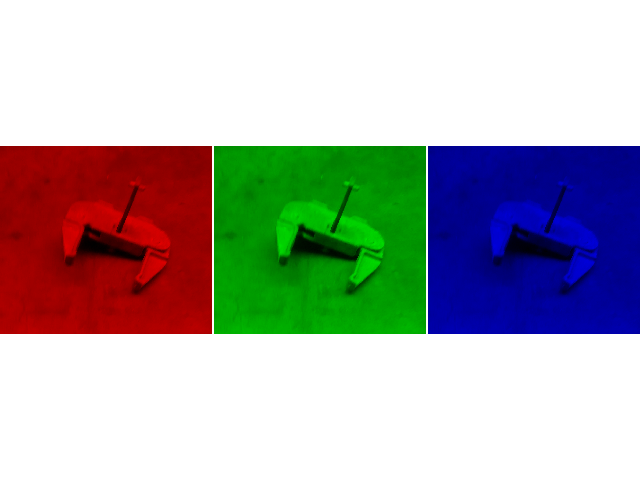
\includegraphics[width=1.7\textwidth]{1rgb.png}};
\end{tikzpicture} 
\end{figure}
\end{frame}

\section{Approach \& Lessons Learned}
\begin{frame}
\begin{center}
\begin{figure}

\begin{tikzpicture}
  [
    chronos={%
      width=120mm,
      height=10pt,
      start date=2017-01-01,
      %start date=2017-08-01,
      end date=2019-01-20,
      %end date=2018-12-31,
      period/.style={draw=green},
      event line/.append style={draw=blue},
      period event line/.append style={draw=green},
      event/.append style={fill=blue!25, draw=blue, text=blue},
      period event/.append style={fill=green!25, draw=green!75!black, text=green!75!black},
    }
  ]
  \chronosperiod [draw=red] {2017-09-04} [draw=red] {2017-11-20} [fill=red!25, draw=red, text=red] {Period P1: \\ Data acquisition, first models, \\ 80\% accuracy} (70pt+.5*\chronosheight)
  \chronosevent [] {2017-09-04} [] {Acquire first batch of images} (-50pt-.5*\chronosheight)
  \chronosevent [] {2017-09-13} [] {Cropping first batch of Images} (-90pt-.5*\chronosheight)
  \chronosevent [] {2017-08-13} [] {Initial discussion with Jelle} (110pt -.5*\chronosheight)
  \chronosperiod [] {2017-11-21} [] {2018-09-22} [] { Moving, KUL courses, \\ Restart work @ NVISO, Summertime} (-7pt-.5*\chronosheight)
  \chronosperiod [draw=red] {2018-09-23} [draw=red] {2018-11-19} [fill=red!25, draw=red, text=red] {Period P2: \\ Reinstall, Refining, Reporting, \\ 90\% accuracy} (60pt+.5*\chronosheight)
  
\end{tikzpicture}
\end{figure}
\end{center}
\end{frame}


\begin{frame}
\begin{itemize}
 \item Training an image classification Neural Network from scratch needs \textbf{millions} of images and days to weeks of computation time 
 \item In two afternoons I took merely 1434 pictures and don't have a datacenter.
 \item \textbf{solution}: stand on the shoulders of giants $\rightarrow$ \textbf{transfer learning}
  \begin{itemize}
    \item Start from Google-trained InceptionV3 \& Xception Neural Networks
    \item NN weights trained for 
\includegraphics[width=0.3\textwidth]{imagenet.jpg}-1000 project: millions of tagged images.
    \item These networks can categorize 1000 common items very well (80\% accurate)
    \item Fine-tune Neural Network on this specific data set starting with the basemodel weights.
  \end{itemize}
\end{itemize}
\end{frame}

\begin{frame}{Image Augmentation}
\begin{itemize}
  \item Still 1434 pictures is a small dataset for transfer learning with CNNs. 
  \item \textbf{solution:} Image Augmentation - Random modifications of the dataset
  \begin{itemize}
	\item Zoom in
	\item Flip image horizontally 
	\item Flip image vertically 
	\item shift image along x axis
	\item shift image along y axis
	\item rotate image 
	\item Make red, green or blue channel shifts
  \end{itemize}
\end{itemize}
\end{frame}

\begin{frame}{Image augmentation 1, 2.0, 2.1}
\begin{figure}
%remove subfigure captions and additional whitespace
\captionsetup[subfigure]{labelformat=empty,farskip=0pt,nearskip=0pt,captionskip=0pt}
\begin{tabular}{cc}
\mlcell{Item \\1.0} &
\raisebox{-0.5\height}{ %centers the image on the line
\subfloat[]{\includegraphics[width = 0.18\textwidth]{aug1-0_1.png}} 
\subfloat[]{\includegraphics[width = 0.18\textwidth]{aug1-0_2.png}} 
\subfloat[]{\includegraphics[width = 0.18\textwidth]{aug1-0_3.png}}
} \\[-2ex] %removes unnecessary vertical whitespace
\mlcell{Item \\ 2.0} &
\raisebox{-0.5\height}{
\subfloat[]{\includegraphics[width = 0.18\textwidth]{aug2-0_1.png}} 
\subfloat[]{\includegraphics[width = 0.18\textwidth]{aug2-0_2.png}} 
\subfloat[]{\includegraphics[width = 0.18\textwidth]{aug2-0_3.png}}
} \\[-2ex] %removes unnecessary vertical whitespace
\mlcell{Item \\ 2.1} &
\raisebox{-0.5\height}{
\subfloat[]{\includegraphics[width = 0.18\textwidth]{aug2-1_1.png}} 
\subfloat[]{\includegraphics[width = 0.18\textwidth]{aug2-1_2.png}} 
\subfloat[]{\includegraphics[width = 0.18\textwidth]{aug2-1_3.png}}
} \\
\end{tabular}
\end{figure}
\end{frame}

\begin{frame}{Image augmentation 3, 4.0, 4.1}
\begin{figure}
%remove subfigure captions and additional whitespace
\captionsetup[subfigure]{labelformat=empty,farskip=0pt,nearskip=0pt}
\begin{tabular}{cc}
\mlcell{Item \\1.0} &
\raisebox{-0.5\height}{ %centers the image on the line
\subfloat[]{\includegraphics[width = 0.18\textwidth]{aug3-0_1.png}} 
\subfloat[]{\includegraphics[width = 0.18\textwidth]{aug3-0_2.png}} 
\subfloat[]{\includegraphics[width = 0.18\textwidth]{aug3-0_3.png}}
} \\[-2ex] %removes unnecessary vertical whitespace
\mlcell{Item \\ 2.0} &
\raisebox{-0.5\height}{
\subfloat[]{\includegraphics[width = 0.18\textwidth]{aug4-0_1.png}} 
\subfloat[]{\includegraphics[width = 0.18\textwidth]{aug4-0_2.png}} 
\subfloat[]{\includegraphics[width = 0.18\textwidth]{aug4-0_3.png}}
} \\[-2ex] %removes unnecessary vertical whitespace
\mlcell{Item \\ 2.1} &
\raisebox{-0.5\height}{
\subfloat[]{\includegraphics[width = 0.18\textwidth]{aug4-1_1.png}} 
\subfloat[]{\includegraphics[width = 0.18\textwidth]{aug4-1_2.png}} 
\subfloat[]{\includegraphics[width = 0.18\textwidth]{aug4-1_3.png}}
} \\
\end{tabular}
\end{figure}
\end{frame}

\begin{frame}{Training CNNs is a probabilistic process}
\begin{itemize}
 \item Training Neural Networks is probilistic process, it contains random variables. 
 \item Train the same model twice, it will have different results 
 \item \textbf{How to compare different models?}
\end{itemize}
\end{frame}

\begin{frame}{LL:5-fold cross-validation}
\begin{figure}
For each model run 5 experiments
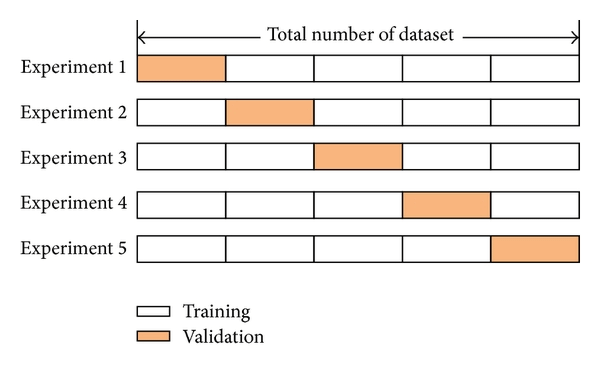
\includegraphics[width=0.8\textwidth]{5foldCV} \\
And average over the 5 different experiments. 
%And reference it from researchgate.net
\end{figure}
\end{frame}

\begin{frame}{Hardware \& Software Stack}
\begin{table}
\begin{tabular}{r|cc}
& Period 1 & Period 2 \\ \hline
Keras &  2.0.6 & \textbf{2.2.2} \\
Tensorflow & 1.3.0 & \textbf{1.13.0} \\
Python & 3.6 & 3.6 \\
cuDNN & 5.1 & \textbf{7.0} \\ 
CUDA & 8.0 & \textbf{9.0} \\
Ubuntu & 16.04.3 LTS & \textbf{fresh 16.04.3 LTS} \\
Storage & Seagate 3TB-7600RPM & \textbf{Samsung 265GB SSD} \\
NVIDIA GPU & \multicolumn{2}{c}{GTX 1060 6GB} \\
Intel CPU &  \multicolumn{2}{c}{Core i5-3570K CPU \@ 3.40GHz} \\
RAM & \multicolumn{2}{c}{16 GB} \\
\end{tabular}
\caption{In P1 trained with testfiles on HDD, later in P2 reinstalled full software stack, with updated libraries, on new SSD}
\end{table}
\end{frame}

\begin{frame}{LL: Disk speed/Library version matters}
\begin{table}
\caption{Rough estimate: Factor 10 training speed improvement in Period 2}
\begin{tabular}{ccccc}
Period & Experiment ID & \mlcell{Approximate \\ Training \\ Hours} & \mlcell{Best Validation \\ Loss (lower = better)} \\ \hline
1 & mXc\_v5\_split0 & $7$ & $0.17$ \\
1 & mXc\_v6\_split0 & $7$ & $0.2$ \\
1 & mXc\_v5\_split2 & $7$ & $0.16$ \\
1 & mXc\_v6\_split2 & $7$ & $0.18$ \\
2 & mXc\_v5\_split0 & $0.6666$ & $0.25$ \\
2 & mXc\_v6\_split0 & $0.6500$ & $0.22$ \\
2 & mXc\_v5\_split2 & $0.5833$ & $0.2$ \\
2 & mXc\_v6\_split2 & $0.6666$ & $0.22$ \\
\end{tabular}
\end{table}
\end{frame}


\begin{frame}{LL: Signal/Noise matters}
\begin{itemize}
 \item If $\frac{signal}{noise}$ of image is too large, CNN have hard time picking up on the signal.
 \item I learned it the hard way:
\begin{itemize}
 \item First trained model with 675 uncropped rectangular images. \\ $\Rightarrow$ Poor training results.
 \item After 1,5h of cropping 675 images and retraining the network using Cropall tool %TODO:add ref
  \\ $\Rightarrow$ Better results ~80\% accuracy?
\end{itemize}
\end{itemize}
\end{frame}

\begin{frame}{LL: uncropped vs cropped}
\begin{tabular}{cc}
uncropped & cropped \\
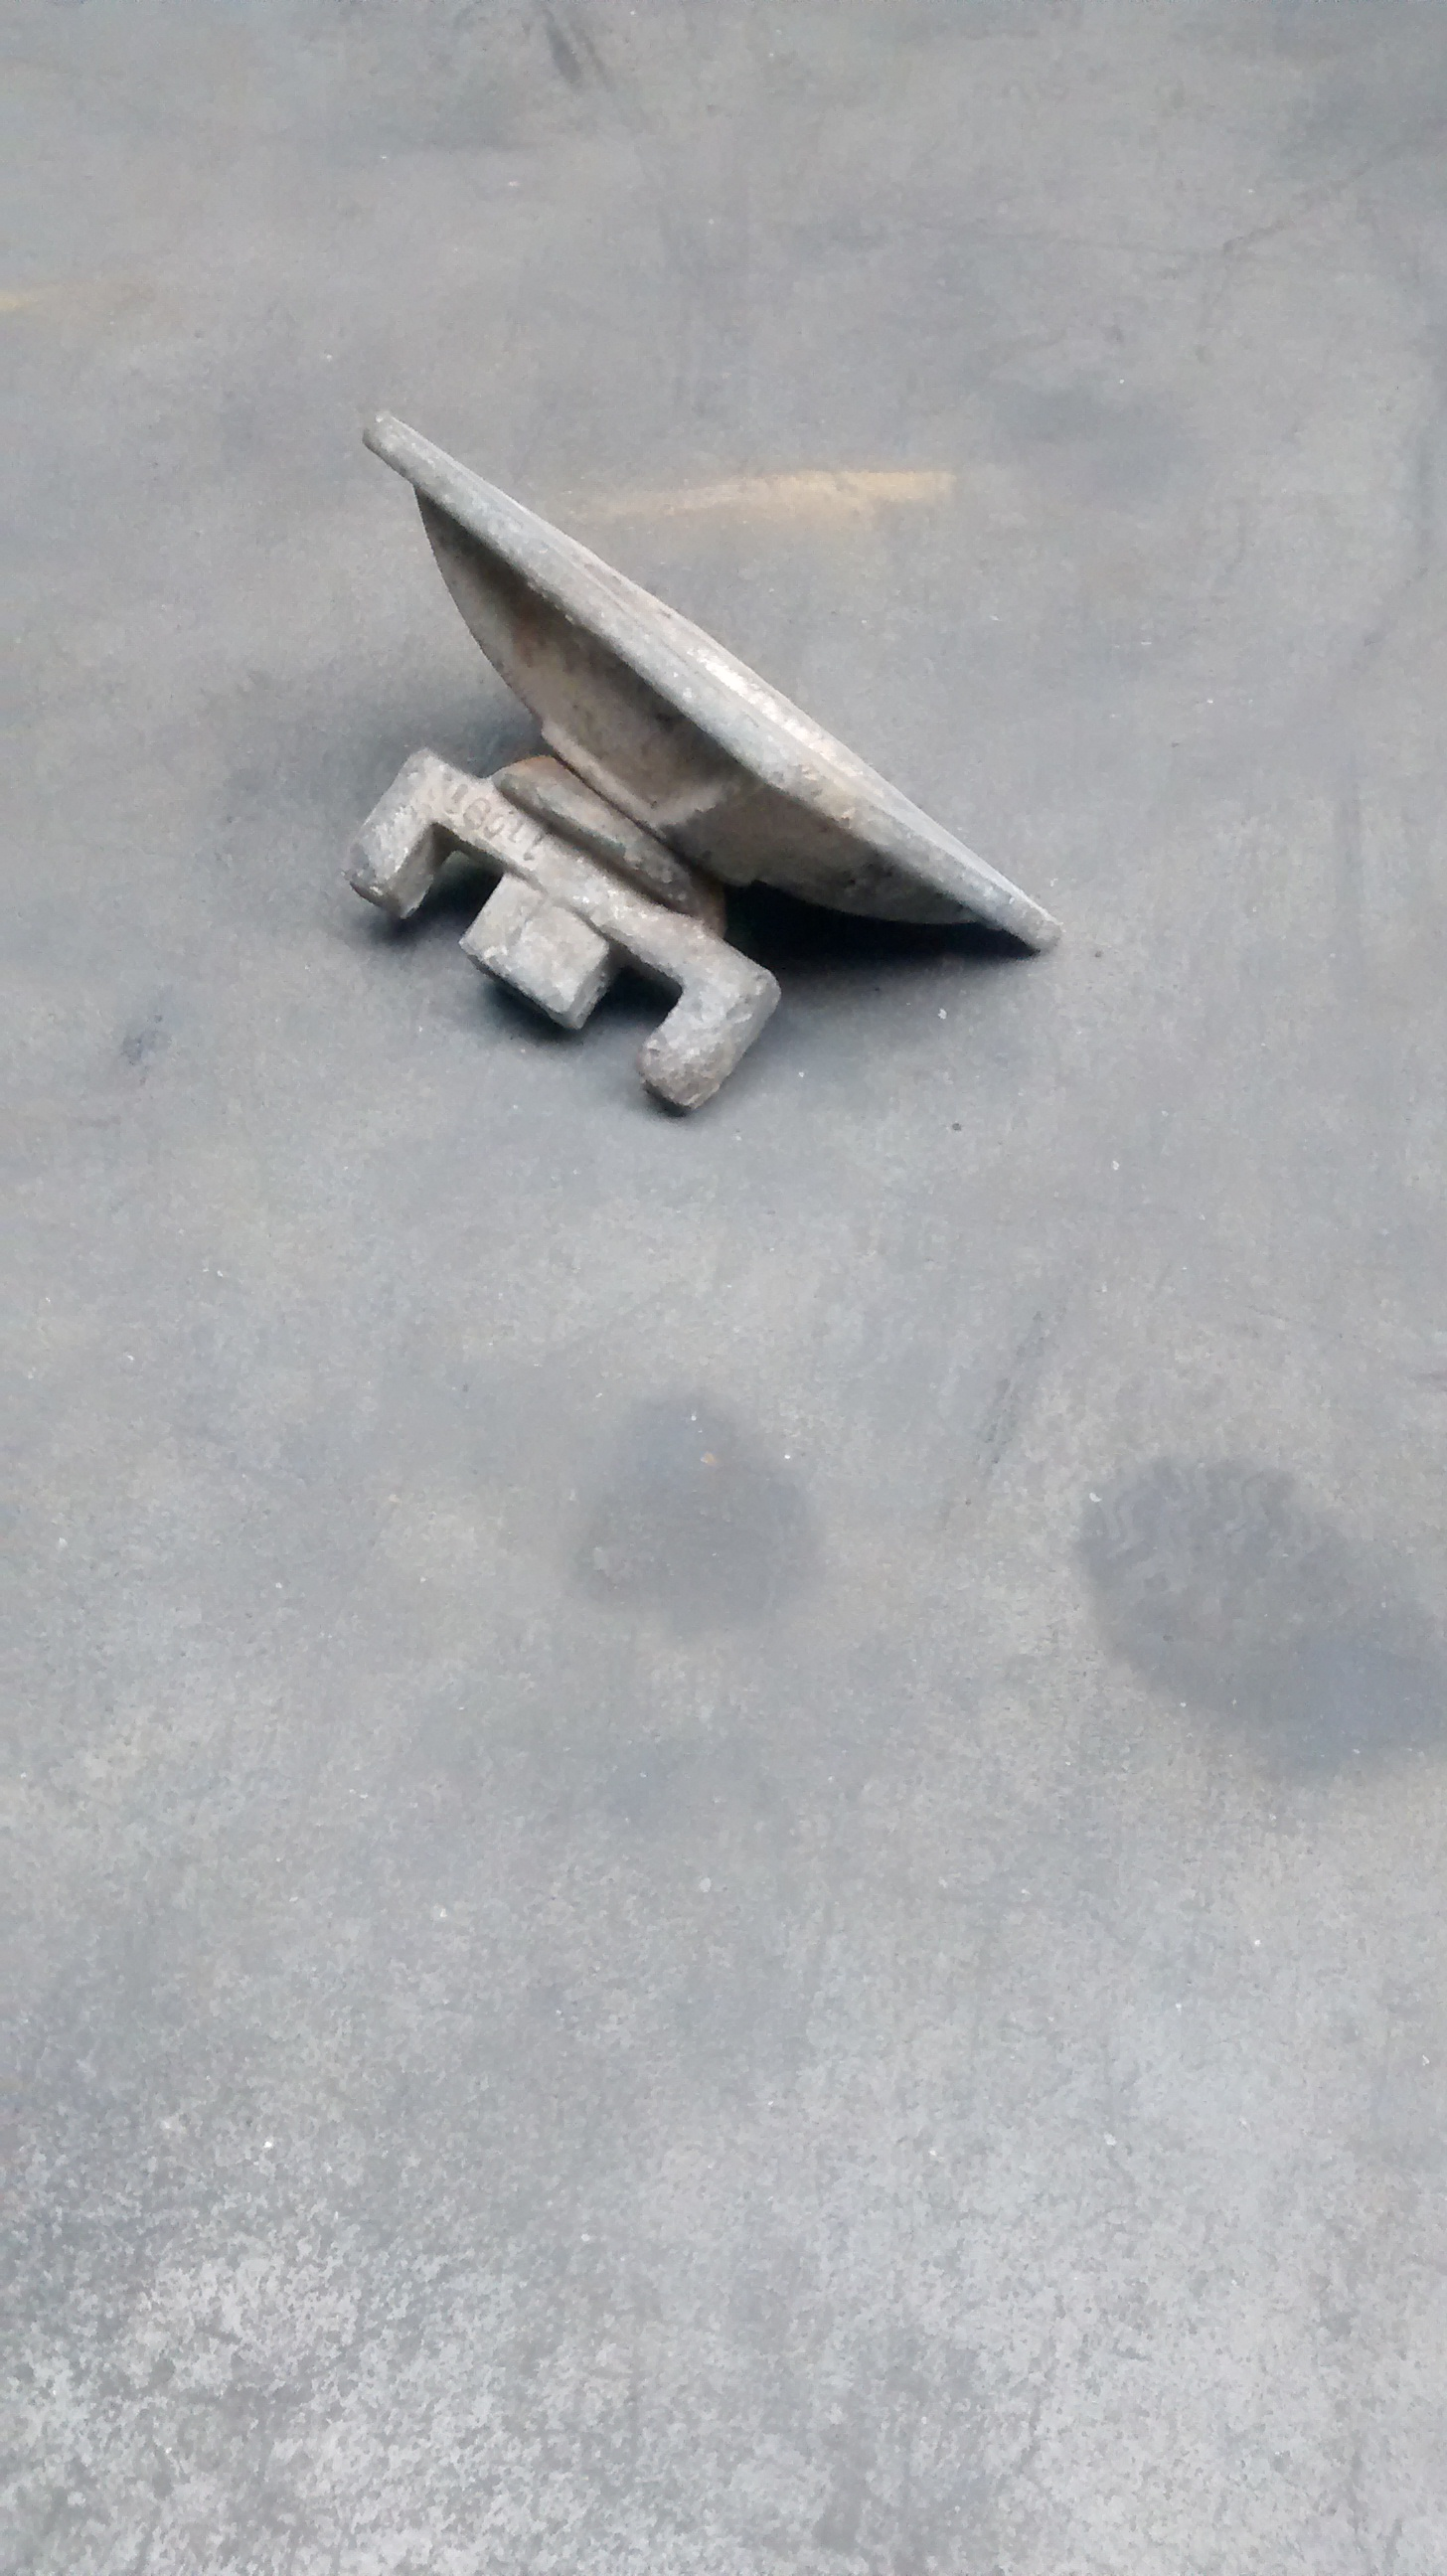
\includegraphics[width=0.4\textwidth]{2_1uncrop.jpg} 
& \raisebox{0.5\height}{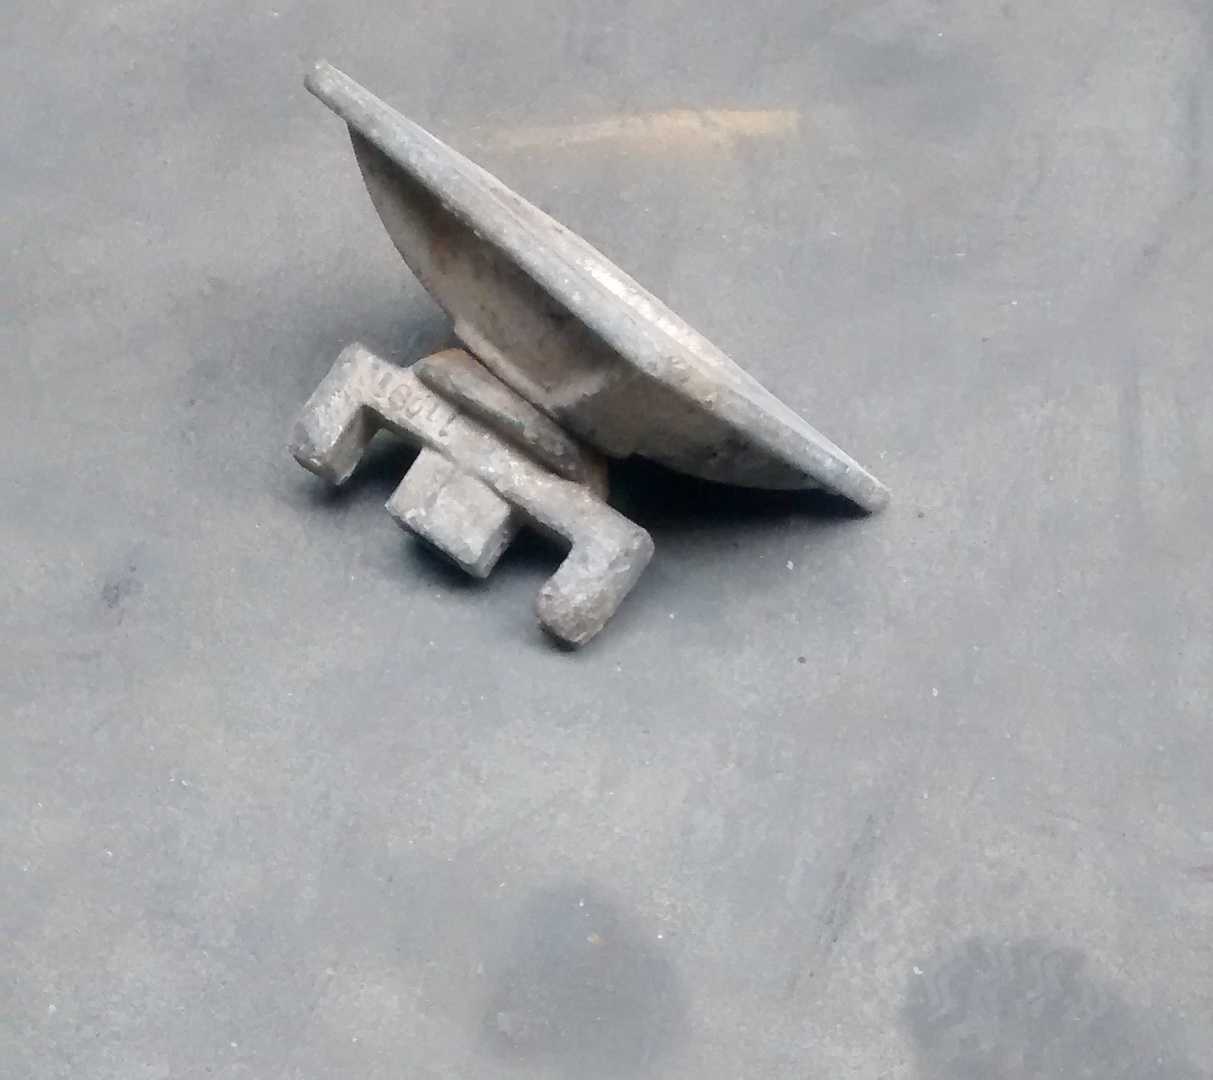
\includegraphics[width=0.4\textwidth]{2_1crop.jpg}} \\
\end{tabular}
\end{frame}

\begin{frame}{LL: I learned a lot!}
\begin{itemize}
 \item Setting up a Graphics Processing Unit CNN training machine (twice). 
 \item Using state of the art CNN libraries
 \item Improved python scripting 
 \item Learned a lot about Neural Networks and Machine Learning 
 \item Read many academic papers, books, blogs, \ldots 
\end{itemize}
\huge{For me the project was a huge success!}
\end{frame}



\section{Results}
\begin{frame}
\begin{tabular}{cc}
\mlcell{Validation \\ Loss} &
\raisebox{-0.5\height}{
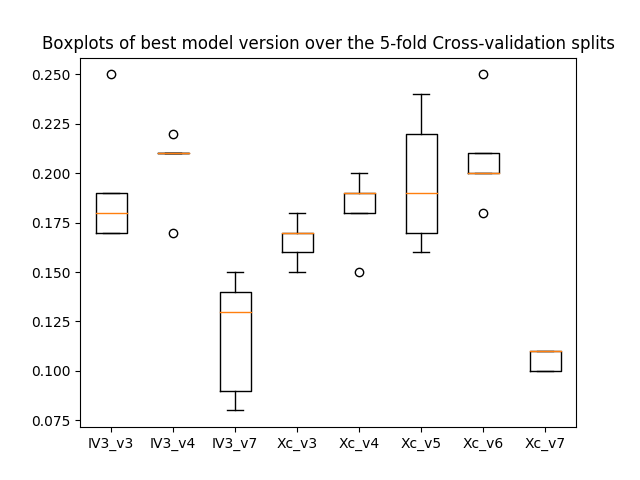
\includegraphics[width=0.9\textwidth]{boxplots.png}
}\\
& basemodel: IV3\_ = InceptionV3, XC\_ = Xception \\
\end{tabular}
\end{frame}

\begin{frame}{Best Model}
\begin{itemize}
 \item Best model is Xc\_v7
  \begin{itemize}
    \item Has Xception with ImageNet weights as basemodel.
    \item Fully-connected penultimate layer of 256 neurons.
    \item Was optimized with Stochastic Gradient Descent first and the Adam optimizer finally. 
  \end{itemize}
 \item Has average validation loss of $0.1011802$ \\ $\Rightarrow$ validation accuracy of $ 1 - 0.1011802 = 0.8988198 \approx 90\%$
\end{itemize}
\end{frame}

\begin{frame}{Caveat}
Note that while 90\% accuracy seems impressive this is still a very limited dataset.
There is no guarantee that the model will perform as well with images taken today.
Models CAN degrade over time and are biased by the dataset they are trained on.
\end{frame}

\section{Future Work}
\begin{frame}{Advice}
\begin{itemize}
  \item Create Image Capture Pipeline
  \item For CNNs: more data, better results
  \item Multiple-camera's $\rightarrow$ vote per camera
  \begin{itemize}
  \item Upside: Will likely improve accuracy, more camera's == more data
  \item Downside: Processing multiple images fast enough might be a challenge 
  \end{itemize}
  \item Deploy current best model and monitor whether performance degrades?
\end{itemize}
\end{frame}{}

\begin{frame}{CNN Technical}
\begin{itemize}
 \item Multiple-cameras will give more reliable detection.
  \begin{itemize}
  \item Upside: Will likely improve accuracy, more camera's == more data
  \item Downside: Processing multiple images fast enough might be a challenge 
  \end{itemize}
 \item Adding depth sensor (e.g. Microsoft Kinect sensor) will likely improve accuracy 
  \begin{itemize}
  \item Upside: Will likely improve accuracy 
  \item Downside: transfer learning not yet possible, long training times, $\frac{signal}{noise}?$
  \end{itemize}
 \item Exploring 3D renderings of the CAD files could help recognition.
    \begin{itemize}
      \item Even low fidelity renderings have shown to help train Neural Networks
      \item Upside: CAD files of all items exist already.
      \item Downside: Rendering also costs computation time. 
    \end{itemize}
 \item Generate more data synthetically using Generative Adverserial Neural Networks
    \begin{itemize}
      \item Advanced form  of image augmentation 
      \item Upside: Could significantly improve robustness and accuracy 
      \item Downside: Technically challenging, high computation time cost 
    \end{itemize}
\end{itemize}
\end{frame}

\begin{frame}{Project} \begin{itemize}
 \item Consider collaboration with University.
 \item Master Artificial Inteligence is booming
  \begin{itemize}
  \item Internship students could help create the machine learning pipeline.
  \item Partnership with industry is highly encouraged
  \item  
  \end{itemize}
 \item Depth sensor (e.g. Microsoft Kinect sensor) will improve accuracy 
  \begin{itemize}
  \item Transfer learning not possible
  \item 
  \end{itemize}
 \item Using renderings of the CAD files could help in generalisation.
\end{itemize}
\end{frame}

\section{Q\&A}
\begin{frame}
  \begin{itemize}
	    \item How does the system compare to human classification?
	    \item Speed (vs 24/7), cost (long-term cost hard to estimate, software and model maintenance), effort, \emph{accuracy}, FP vs FN
	    \item TEST
  \end{itemize}
\end{frame}


\end{document}
